\chapter{Backend}
\label{cha:backend}
Das Backend bezieht sich auf den in Python geschriebenen Teil, welcher
öffentlich nicht zugreifbar ist.
Im folgenden werden die zentralen Module aufgelistet, welche in eine
Beschreibung ihrer Funktion, einer Schnittstellenbeschreibung sowie
teilweise einer Begründung aufgeteilt sind.
Die Schnittstellenbeschreibungen sind dabei in englisch kommentierten Python Methoden-Beschreibungen gefasst. 

\section{Testfälle}
Als Testmethode werden Unit-Tests herangezogen, die mit dem bei Python mitgelieferten Frameworks \texttt{unittest}
ausgeführt werden können. Dabei enthält jedes File den dazugehörigen Testcode, welcher durch direktes Aufführen des
.py files ausgeführt wird:

\begin{lstlisting}[language=Python]
# Eigentlicher Source
class XYZ:
    def DoSomething(self, param):
        ...

# Abgetrennter Testcode
if __name__ == '__main__'
   import unittest

   class TestXYZ(unittest.TestCase):
       def TestDoSomething(self):
           ...

   unittest.main()
\end{lstlisting}


\newpage
\section{Programmablauf} 
\label{sec:programmablauf}
\begin{figure}[h]
\centering
\label{dia:design:backend:overview}
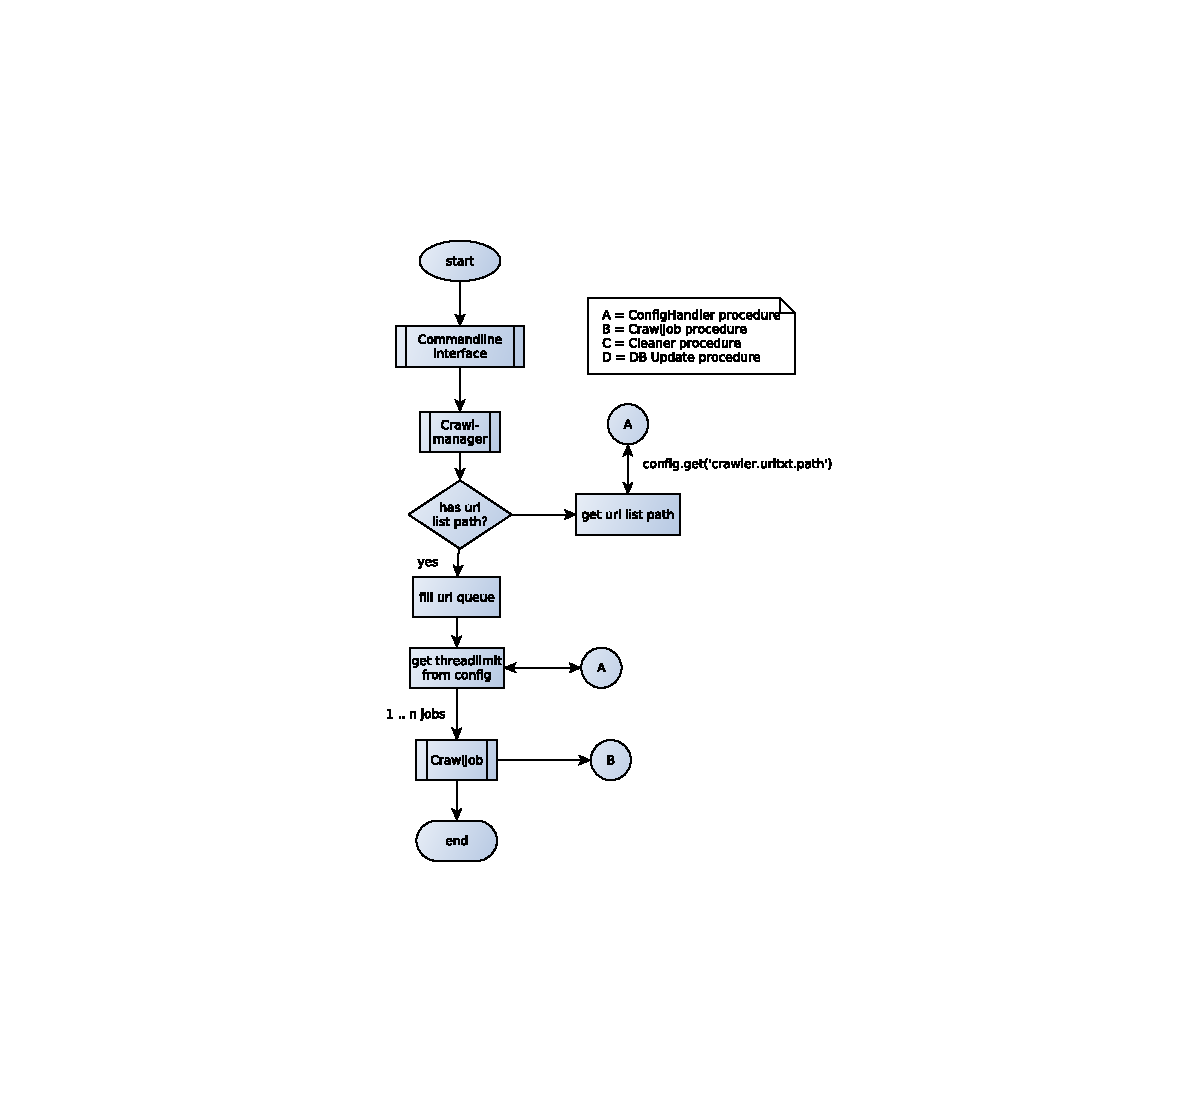
\includegraphics[width=\textwidth]{design/backend/gfx/backend_procedure.eps}
\caption{Ablaufprozedur Backend}
\end{figure}


% section programmablauf (end)

\section{Zentrale Module} 
\label{sec:zentrale_module}

\subsection{ConfigHandler}
\label{sub:confighandler}
\paragraph{Ablauf:}
\label{par:ablauf_}
Grundlegender Ablauf beim Lesen von Configwerten:
\begin{figure}[h]
	\centering
	\label{dia:design:backend:overview}
	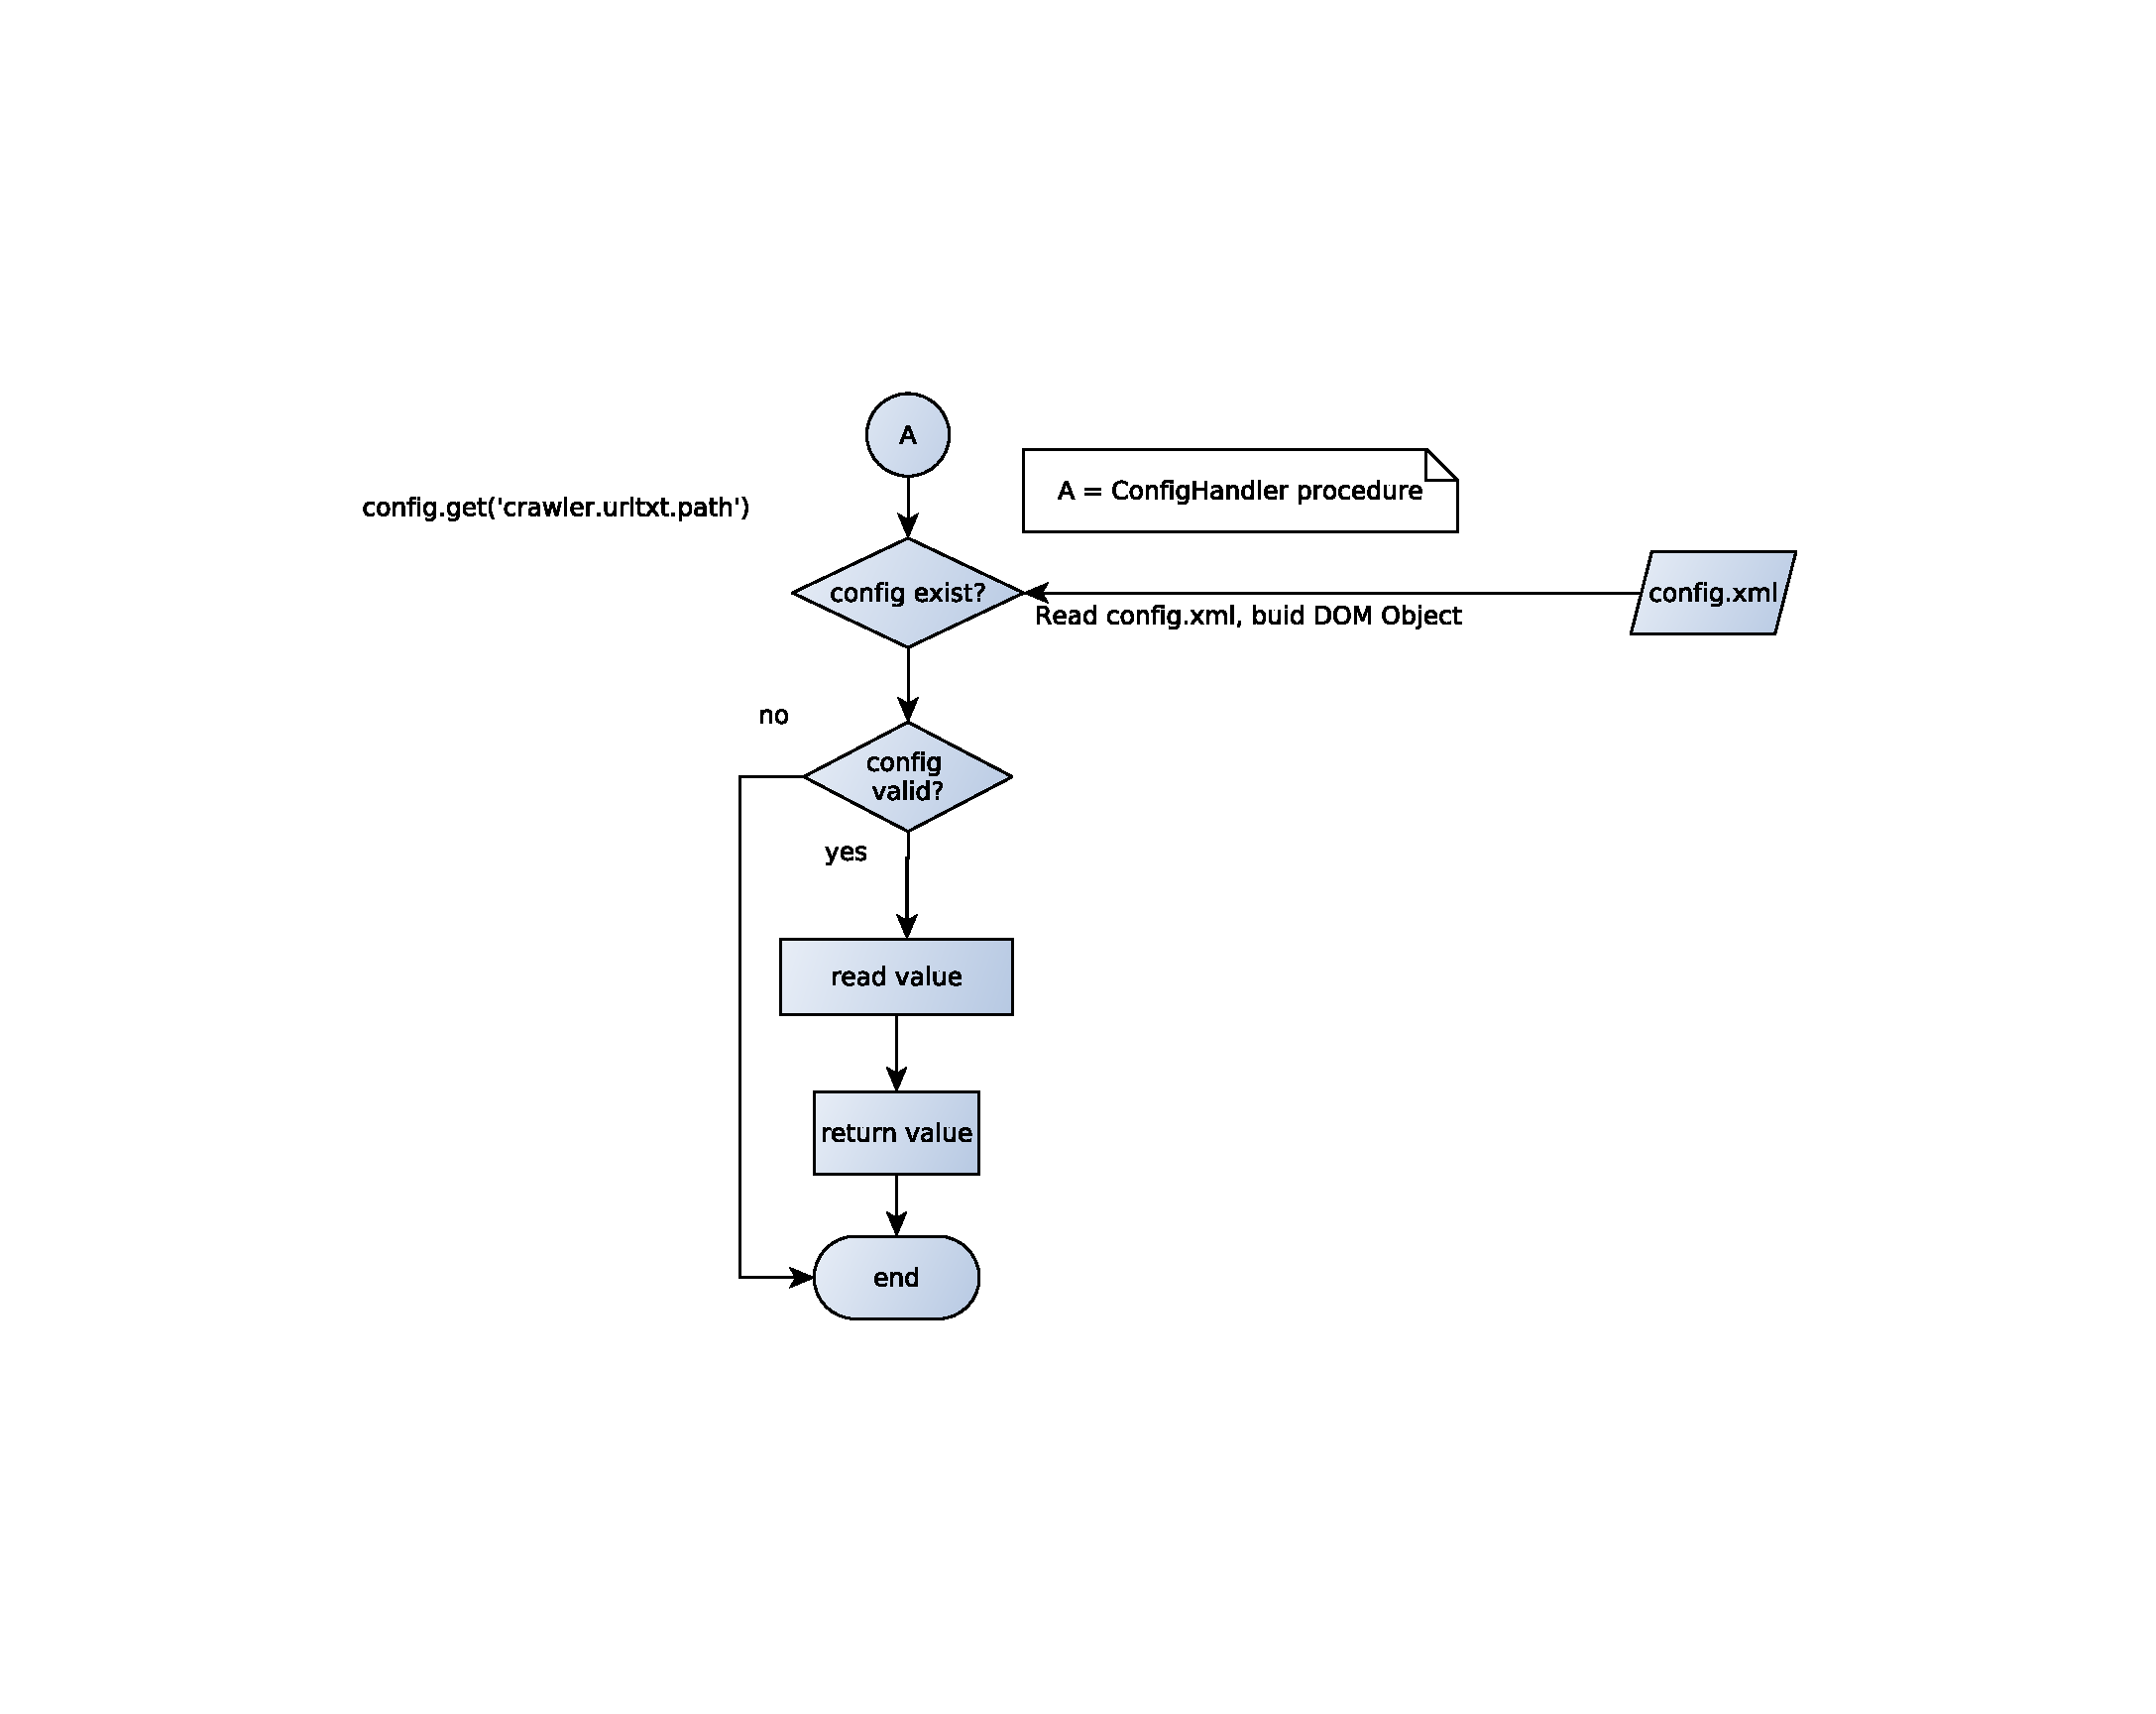
\includegraphics[width=\textwidth]{design/backend/gfx/getting_value.eps}
	\caption{Werte aus der Konfigurationsdatei holen}
\end{figure}

% paragraph ablauf_ (end)
\paragraph{Beschreibung:}
(Entsprechend: \ref{spec:conf})
\label{par:beschreibung_}
Dieser wird zum Lesen und Setzen der Konfigurationswerte verwendet. Die Konfigurationsdatei ist in 
\paragraph{Schnittstelle:}
\label{par:schnittstelle_}
Xml geschrieben und hat folgenden Aufbau:
    \lstinputlisting[language=XML,basicstyle=\ttfamily\fontsize{8}{10}\selectfont]{../../conf/webarchive.conf.xml}
Der Zugriff auf bestimmte Werte ist nach Domainprinzip aufgebaut, so
lässt sich der Wert ,,Serverport'' über eine Punkt-separierte ,,URI'' auslesen: \texttt{webarchive.server.port} 
\\ \\
Der erste Knoten \texttt{webarchive} ist stets vorhanden, und kann daher optional ausgelassen werden.

\paragraph{Begründung/Hintergrund:}
\label{par:begr_ndung}
Das relativ einfache URI Prinzip wurde gewählt um stets einen direkten
Bezug zwischen der XML Struktur und den abgefragten Werten herzustellen.
\\
In späteren Versionen ist folgende Erweiterun denkbar: Statt die
Default-Werte fest in den Programmcode zu legen, wird eine systemweite
und immer verfügbare config.xml angelegt, auf die zurückgefallen werden
kann.

% paragraph begr_ndung (end)


\subsection{Commandline Interface}
\label{sub:commandline_interface}
\paragraph{Beschreibung}
\label{par:beschreibung}
Dieses Interface realisiert die zentralle Administrationsschnittstelle zum Webarchiv. 
Das Interface soll dabei ähnlich wie git nach dem folgenden Schema funktionieren:
\begin{verbatim}
archive [--general-options] submodule [--arguments-specific-to-submodule]
\end{verbatim}
submodule kann dabei einer der folgenden Module sein:
\begin{table}[h]
\centering
\begin{tabular}{|l|l|}
    \hline
        init & Initialisiert ein leeres archiv an einem bestimmten Pfad \\
    \hline
        crawler & Zugriff auf Starten und Stoppen des Crawlvorgangs \\
    \hline
        javadapter & Starten und Stoppen der Java Schnittstelle \\
    \hline
    db & Bietet Funktionen um die Datenbank neu zu generieren
    (entspricht: \ref{req:Db:recovery}) \\
    \hline
        config & Bietet Zugriff um Werte aus der config zu holen oder zu überschreiben
        (entspricht: \ref{req:Cr:cmd:overwrite}) \\
    \hline
\end{tabular}
\end{table}

\paragraph{Begründung/Hintergrund:}
\label{par:begr_ndung_}
Es wurde sich für ein einfaches Commandline Interface entschieden, da
Kenntnisse im Umgang mit der Unix-Shell auf der User Seite vorrausgsetzt
werden.

% paragraph begr_ndung_ (end)

\subsection{Initialisierung} 
\label{sub:initialisierung}
\paragraph{Beschreibung:}
\label{par:beschreibung}
% paragraph beschreibung (end)
Durch dieses Modul wird ein leerer Archivordner erstellt, der lediglich
ein Default-Configtemplate mit dem Pfad zum Archiv enthält, sowie einen leeren Ordner ,,content'',
in dem später die Crawldaten abgelegt werden.
Weitere Einstellung müssen händisch in der Config nachgetragen werden.
\\
Angelegt wird der Ordner über %\verbatim{archive init /pfad/zum/archive}
\paragraph{Schnittstelle:}
\label{par:schnittstelle}
\begin{lstlisting}[language=python]
def init_archive(path = '.'):
    """
    Initializes empty archive structure with default Config
    at ,,path'' with the following structure:

      archive/
        content/ 
           # empty
        webarchive.config.xml
    """
    pass
\end{lstlisting}

\paragraph{Begründung:}
\label{par:begr_ndung_}
Das Anlegen des Archiv-Ordners wurde nicht dem Nutzer überlassen, da
Fehler hierbei sich auf die spätere Funktionsweise auswirken können.
% paragraph begr_ndung_ (end)


% paragraph schnittstelle_ (end)
\subsection{Crawlermanager}
\label{sub:crawlermanager}
\paragraph{Beschreibung:}
\label{par:beschreibung_}
% paragraph beschreibung (end)
Der Crawlermanager liest eine Liste mit URLs aus einer Datei, die entweder auf der Kommandozeile oder in
der Config definiert wurde. Die URLs sind in diese Datei zeilenweise einzutragen und können durch ein \# auskommentiert werden.
Über einen ThreadPool wird dann für jede URL ein Crawljob gestartet. Die maximale Anzahl der dabei laufenden Crawljobs wird bei
der Instanzierung des ThreadPools aus der Config gelesen.
\\
Desweiteren hat der Crawlermanager nur administrative Funktionen wie dem Stoppen der laufenden Crawljobs.
\paragraph{Schnittstelle:}
\label{par:schnittstelle_}
Prinzipieller Aufbau des Crawlmanagers:
% paragraph schnittstelle_ (end)
\begin{lstlisting}[language=python]
class CrawlManager:
    def __init__(self):
        """
        Instance a new CrawlerManager,
        which must be started via start()
        """
        pass

    def start(self):
        """
        Reads configured URLs from Config, and start a new job for each
        """
        pass

    def shutdown(self,hard=False): 
        """
        Shuts down currently running crawljobs
        If hard is set to True, currently running jobs
        are canceled immediately, instead of syncing already
        gathered data to archive.
        """
        pass

    def reload(self):
        """
        Reloads configured URLs and replaces current Queue with new URLs.
        Leaves running Jobs untouched.
        """
        pass

\end{lstlisting}

\newpage
% paragraph api_ (end)
\subsection{Crawljob}
\label{sub:crawljob}
\paragraph{Ablauf:}
\label{par:ablauf_}
\begin{figure}[h]
	\centering
	\label{dia:design:backend:overview}
	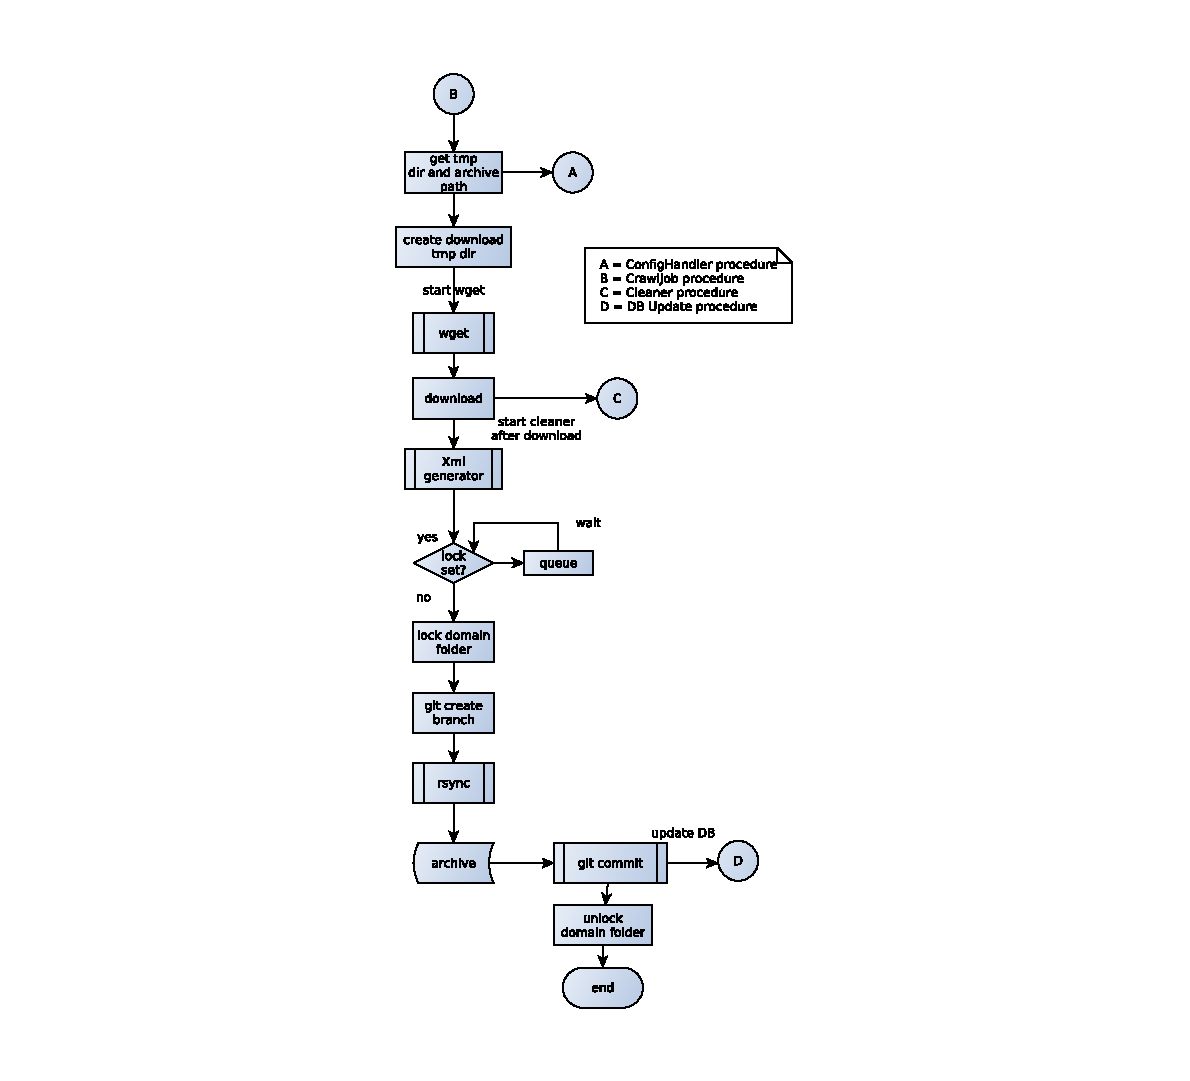
\includegraphics[width=\textwidth]{design/backend/gfx/crawljob.eps}
	\caption{CrawlJob Prozedur}
\end{figure}


% paragraph ablauf_ (end)

\paragraph{Beschreibung:}
\label{par:beschreibung_}
Der Crawljob ist ein autonomer Thread der die unten aufgelisteten Submodule beeinhaltet.
Bevor die einzelnen Submodule abgearbeitet werden, wird ein temporäres Arbeitsverzeichnis angelegt.
Die Lage dieses Verzeichnisses kann in der Config festgelegt werden.
\paragraph{Schnittstelle:}
\label{par:api_}

\begin{lstlisting}[language=python]
class CrawlJob():
    def __init__(self, ident, url):
        """
        Gets Identity and Url that should be crawled,
        Identity is needed to generate tmp folder
        """
        pass

    def shutdown(self, hard=False): 
        """
        Shuts down currently running crawljob
        If hard is set to True, currently running job
        is canceled immediately, instead of syncing already
        gathered data to archive.
        """
        pass
\end{lstlisting}
\paragraph{Begründung/Hintergrund:}
\label{par:begr_ndung_hintergrund_}
Ein ,,Wget-Wrapper'' wird zum Crawlen verwendet, da wget alle vom iisys benötigten Funktionalitäten bietet und
in der kürze der Zeit kein gleichwertiger Ersatz implementierbar ist. Um das Crawlen global zu 
beschleunigen wurde dieses ,,parellisiert'', es werden hier einfach mehrere Wget-Wrapper Instantzen gestartet.
Um die Gesamtgeschwindigkeit des Systems zu steigern wird ebenfalls empfohlen die ,,tmp''-Crawlordner auf ein
ramfs zu legen.

\subsubsection{Wget}
\label{ssub:wget}
\paragraph{Beschreibung:}
\label{par:beschreibung_}
% paragraph beschreibung_ (end)
Eine Managementschicht zur Abstraktion von wget.
Dieser wird eine Domain zugeteilt welche von wget mit konfigurierbaren Parametern gecrawlt wird.
Die allgemeine Webseitenstruktur wird dabei intakt gelassen:

\begin{verbatim}
    www.heise.de/
        index.html
        news/
            newsfeeds.html
            favicon.png
        ...
\end{verbatim}

\paragraph{Schnittstelle:}
\label{par:schnittstelle_}

\begin{lstlisting}[language=python]
class Wget():
    def __init__(self, tmpfolder, url):
        """
        Instance a new Wget Wrapper,
        which must be started with start()

        tmpfolder: The folder where the downloaded data will be stored
        url: The url you want to be crawled recursively
        """
        pass

    def start(self): 
        """
        Start crawling the URL in the background,
        the function returns immediately
        """
        pass

    def stop(self):
        """
        Stop a running wget instance
        If start() was not called, or finished already,
        this function is a No-op
        """
        pass
\end{lstlisting}


% paragraph begr_ndung_hintergrund_ (end)
% paragraph schnittstelle_ (end)
\subsubsection{Cleaner}
\label{ssub:cleaner}
\paragraph{Beschreibung:}
\label{par:beschreibung_}
Der Cleaner bereingt die Verzeichnisstruktur indem er leere Ordner und Dateien löscht.
Desweiteren wird folgende Restrukturierung durchgeführt:
\begin{verbatim}
    www.heise.de/ 
        index.html/
            data
        news/
            newsfeeds.html/
                data
            favicon.png/
                data
        ...
\end{verbatim}


\begin{itemize}
    \item Ordner werden intakt gelassen
    \item Für jede reguläre Datei wird ein gleichnamiges Verzeichnis angelegt
    \item Die regulären Daten werden in dieses Verzeichnis mit den Namen ,,data'' verschoben.
\end{itemize}

Außerdem werden während des Strukturierens die grundlegenden Metadatan als Liste im Speicher gesammelt.
Bevor die Datei an das Filtersystem weitergeleitet wird, wird ein ,,Titel'' abhängig vom MIME-Type ermittelt.
Pro Datei werden die konfigurierten Filter ausgeführt, welche entscheiden ob eine Datei gelöscht werden soll oder nicht.
Gibt ein Filter ,,false'' zurück, so wird der jeweilige Dateiordner samt Inhalt sowie die Metadatan gelöscht,
ohne dass weitere Filter aufgerufen werden müssen.
\\
Die gesammelten Metadaten werden in einem Metadatenobjekt gesammelt. Die gesammelten Daten entsprechen dabei 
der Liste aus \ref{spec:model} abzüglich der ,,commitTime'', da diese erst beim Check-In erhoben wird.

\paragraph{Schnittstelle:} 
\label{par:schnittstelle_}
\begin{lstlisting}[language=python]
class Cleaner():
    def __init__(self, path):
        """
        Instance a new cleaner, which is
        supposed to cleanup recursively in ,,path''
        """
        pass

    def restructure(self): 
        """
        Traverse the filetree and restructure
        it as described above.
        """
        pass
  
    def cleanup(self):
        """
        Remove emtpy files and directories
        in ,,path'' recursively
        """
        pass
\end{lstlisting}

\paragraph{Begründung/Hintergrund:}
\label{par:hintergrund_}
Beim Cleaner wird auf das Unix Tool ,,find'' zugegriffen. Dieses eignet sich aufgrund einer Vielzahl
von Optionen und der Möglichkeit weitere ,,Kommandos'' zu übergeben, gut dazu eine Ordnerstruktur rekursiv
zu durchlaufen und leere Dateien und Ordner zu löschen.

% paragraph hintergrund_ (end)

% paragraph schnittstelle_ (end)
\subsubsection{Filtersystem}
\label{ssub:filtersystem}
\paragraph{Beschreibung:}
\label{par:beschreibung_}
Gemäß \ref{req:Fi:interface} wird ein Filtersystem für gecrawlte Daten
implementiert.

\begin{description}
  \item[Initialisierung] Bei jedem Cleanup-Vorgang werden alle .py files
    aus dem konfigurierte Filter-Verzeichnis in eine Liste eingelesen
  \item[Filtervorgang] Für jede reguläre Datei wird die Liste mit dem
    Filtern durchlaufen. Die einzelnen .py files werden in einem
    Subinterpreter gestartet, und ihnen wird eine Kopie des
    Metadaten-Dictionaries des entsprechenden Files mitgegeben
    \texttt{filter\_input}.
  \item[Auswertung] Jeder Filter bekommt zudem eine Boolean-Variable
    \texttt{filter\_result} übergeben, welche anfangs auf \texttt{True}
    gesetzt ist. Will der Filter die Datei aussortieren so setzt er sie
    auf ein unwahren Wahrheitswert. 
  \item[Aussortierung] Gibt der Filter \texttt{False} zurück, so wird
    das Metadaten-Dictionary, sowie der zugehörige Ordner gelöscht. 
    Bei True wird regulär weitergemacht.
\end{description}

\paragraph{Schnittstelle:}
\label{par:schnittstelle_}
Filter werden während des ,,Cleaner'' Vorgangs ausgeführt.
\begin{lstlisting}[language=python]
    # Inside the filter file two additional global variables
    # are defined:
    #     filter_input  : A copy of a metadata dictionary object
    #     filter_result : The decision of the filter is stored here
    #                     by default the decision is True.
    #
    # Note: filter *.py files cannot be run directly, since 
    #       filter_input and filter_result will not be defined there
    #
    # Example:
    if filter_input['mimeType'] == 'image/gif':
        filter_result = False
\end{lstlisting}
% paragraph schnittstelle_ (end)

\paragraph{Begründung:}
\label{par:begr_ndung_}
Die Filter werden in Python kodiert, da dies mit einfachem eingebauten Support für
Dictionaries und Subinterpreter eine optimale Lösung darstellt.
darstellt. Java ist in unsere Augen nicht sinnvoll da einzelne Filter
selten über mehr als 100 Zeilen Quelltext verfügen werden.
% paragraph begr_ndung_ (end)


\subsubsection{Xml Generator}
\label{ssub:xmlgen}
\paragraph{Beschreibung:}
\label{par:beschreibung_}
% paragraph beschreibung_ (end)
Hierbei werden aus der Metadatenliste Xml-Dateien zum jeweiligen Content
geschrieben (\texttt{data.xml}, siehe \ref{spec:xml}) 
Beim Xml generieren werden die Metadaten mit dem aktuellen Systemdatum versehen.
\paragraph{Schnittstelle:}
\label{par:schnittstelle_}

\begin{lstlisting}[language=python]
class XmlGenerator:
    def __init__(self, meta_obj):
        """
        Build a data.xml from a template and the meta_obj dictionary
        """
        pass

    def write(self, path = None):
        """
        Write XML to location ,,path'', 
        if not specified the path from meta_obj is taken

        Throws: IOError on failure
        """
        pass
\end{lstlisting}
% paragraph schnittstelle_ (end)
\paragraph{Begründung/Hintergrund:}
\label{par:begr_ndung_hintergrund_}
Um Schreibzugriffe auf die Festplatte (höchstwahscheinlich langsamste Komponente im System) zu minimieren
und nicht doppelt traversieren zu müssen werden die Metadaten nach dem extrahieren im Speicher gehalten und
erst kurz vor dem Synchronisieren ins Archiv generiert und auf die Festplatte geschreieben. 


% paragraph begr_ndung_hintergrund_ (end)
\subsubsection{DB Generator}
\label{ssub:dbgen}
\paragraph{Beschreibung:}
\label{par:beschreibung_}
Analog zur Xml-Generierung wird ein SQL-Statement erstellt, dass Daten aktualisiert oder neu hinzufügt.
Ist die Datenbank noch nicht vorhanden so wird sie neu erstellt.
% paragraph beschreibung_ (end)

\paragraph{Schnittstelle:}
\label{par:schnittstelle_}
\begin{lstlisting}[language=python]
class DBGenerator:
    def __init__(self, meta_obj_list):
        """
        Build a SQL Query from the meta_obj_list to update and insert new items the Database 
        """
        pass

    def commit(self):
        """
        Send Query to Database,
        this function blocks till finished

        Throws: IOError on failure
        """
        pass
\end{lstlisting}

% paragraph schnittstelle_ (end)

\subsubsection{Rsync}
\label{ssub:rsync}
\paragraph{Beschreibung:}
\label{par:beschreibung_}
Rsync ist eine Managementschicht für das Unix Tool ,,rsync'' \url{http://de.wikipedia.org/wiki/Rsync}. Rsync wird verwendet um die gecrawlten Daten sauber ins Archiv zu synchronisieren.
Hierbei wird der aktuelle gecrawlte Inhalt ins Archiv gespiegelt.
\\
Rsync wird hier direkt auf Systemebene (subprocess.call(['rsync','--archive','--checksum','--delete','src','dest'])) mit den Paramentern
\begin{itemize}
    \item \texttt{[--archive]}, archive mode
    \item \texttt{[--delete]}, nicht mehr vorhandene Dateien werden im Zielverzeichnis gelöscht
    \item \texttt{[--checksum]}, Dateivergleich basiert auf Checksummen, nicht auf Änderungsdatum
\end{itemize}
aufgerufen um die neu gecrawlten Dateien ins Archiv zu ,,spiegeln''.

\paragraph{Schnittstelle:}
\label{par:schnittstelle_}
\begin{lstlisting}[language=python]
class Rsync:
    def __init__(self, path_src, path_dest):
        """
        Instance a new Rsync-Wrapper object,
        which will sync path_src to path_dest
        after calling start_sync() 
        """
        pass

    def start_sync(self):
        """
        Start the synchronisation process,
        this function will block until finished
        """
        pass
\end{lstlisting}

\paragraph{Begründung/Hintergrund:}
\label{par:begr_ndung_hintergrund_}
Rsync wurde gewählt da es sich seit Jahren als Synchronisationstool im Unixbereich bewährt hat.
Da es mit delta files und checksummen arbeitet ist es für den Einsatz eines Archivs optimal.
Durch die Delta-Kodierung/Checksummen wird das Übertragungsvolumen minimiert.

% paragraph begr_ndung_hintergrund_ (end)

\subsubsection{Git}
\label{ssub:git}
\paragraph{Beschreibung:}
\label{par:beschreibung_}
Das Git Modul ist ein Wrapper für das SCM ,,git''. Es wird verwendet um das Archiv mit einer Versionierung auszustatten. Hierzu werden 
die Dateien ins Archiv per Git hinzugefügt, der Stand wird ,,commited''
und der erzeugte Commit wird mit der ,,commitTime'' getaggt.

\paragraph{Schnittstelle:}
\label{par:schnittstelle_}
\begin{lstlisting}[language=python]
class Git:
    def __init__(self, domain):
        """
        The domain is passed in order to identfiy
        the git-repository on which to operate on
        """
        pass

    def checkout(self, branch_name = None):
        """
        'git checkout' a certain branch-name, or 
        'master' when None is given
        """
        pass

    def branch(self, branch_name):
        """
        Create a new branch named 'branch_name'
        """
        pass

    def commit(self, message = 'edit'):
        """
        Does an 'git add .; git commit -am <message>'
        """
        pass
\end{lstlisting}

\paragraph{Begründung/Hintergrund:}
\label{par:begr_ndung_hintergrund_}
Da die Implementierung eines nativen Python Interface zu git selbst mit GitPython
\url{http://gitorious.org/git-python} oder Dulwich \url{http://www.samba.org/~jelmer/dulwich/}
für die uns zu Verfügung stehenden 6 Wochen zu aufwendig ist, wird die Implementierung über
Python\'s subprocess.call() Schnittstelle statt finden. Durch den ,,Proof of concept'' können
erste Erfahrungen mit git als Archivierungssystem gesammelt werden und bei Bedarf eine native Implementierung
umgesetzt werden.


% paragraph begr_ndung_hintergrund_ (end)
\subsection{Logger}
\paragraph{Beschreibung:}
\label{par:beschreibung}


\label{sub:logger}
Der Logger wird für das zentrale Loggen im Backend verwendet. Er implementiert die folgenden Error Level:

\begin{table}[h]
\centering
\begin{tabular}{|l|l|}
    \hline
    \texttt{critical} & Schwere unerwartete Fehler \\
    \hline
    \texttt{error} & Fehler aufgrund von fehlerhaften Eingaben \\
    \hline
    \texttt{warning} & Unkritische Fehler \\
    \hline
    \texttt{info} & Allgemeine Statusinformationen \\
    \hline
    \texttt{debug} & Debug-Informationen für Entwickler \\
    \hline
\end{tabular} 
\end{table}
% paragraph beschreibung (end)


\paragraph{Schnittstelle:}
\label{par:schnittstelle_}

% paragraph schnittstelle_ (end)
Folgende Funktionen werden bereitgestellt:
\begin{lstlisting}[language=python]
def print(severity, *messages):
    """
    Print an Array of messages with a certain severity
    """
    pass

def verbosity(severity):
    """
    Set the verbosity of the program, 

    Passing a severity of 'debug' for example means
    that all messages are printed, while passing 'warning'
    would mean that only Warnings, Errors and Critical Errors 
    are printed.

    This has only effect on terminal output,
    all logmessages will be written to file anyway.
    """
    pass
\end{lstlisting}

\section{Database Recovery} 
\label{sec:database_recovery}
\ref{req:Db:recovery}
Das Recovery-Werkzeug traversiert über alle momentan vorhandenen Domains, und laufen durch die
jeweilige Git-History von hinten nach vorne. Dabei wird aus den XML Metadaten eine neue Datenbank gebildet.
% section database_recovery (end)

\section{Util} 
\label{sec:util}
Das Util Modul stellt verscheidene Funktionen die von mehreren Modulen genutzt werden bereit.
Erwähnenswert ist hier der ,,Lockmechanismus''
auf Dateisystemebene um Daten beim Zugriff auf gemeinsame  Ressourcen zu schützen.

\section{Javadapter} 
\label{sec:javadapter}
Der ,,Javadapter'' stellt eine Schnittstelle zwischen Python und Java dar.
\begin{description}
  \item [Daemon] Er ist als Daemon implementiert, und ist über einen
    definierten Hostname und Port erreichbar (Hier: \texttt{localhost:42421})
  \item [Kommunikation] Jegliche Interaktion erfolgt über ein
    zeilenbasiertes Textprotokoll. Der Client (Hier: Der Java-Server)
    sendet definerte Kommandos, welche mit mit einer Antwortzeile
    und einem abschließenden ,,OK'' oder ,,ACK [FehlerNachricht]''
    beantwortet werden.
  \item [Instanziierung] Der Adapter ist als eigenes Python Modul
    implementiert, und kann über das Commandline-Interface gestartet
    werden.
\end{description}
 
Folgende Kommandos sollen dabei implementiert werden:
Alle Kommandoes nehmen zusätzliche nicht-optionale Argumente die in
eckigen Klammern angegeben sind.
\begin{table}[h]
  \begin{tabular}{|p{4cm}|p{5cm}|p{7cm}|}
    \hline
    \textbf{Kommando} & \textbf{Returnwerte} & \textbf{Beschreibung} \\
    \hline
    \texttt{lock [domain]} 
    & True/False 
    & Lockt eine bestimmte Domain mittels einen Lockfiles 
    \\
    \hline
    \texttt{try\_lock [domain]} 
    & True/False 
    & Wie \texttt{lock}, wartet aber nicht wenn lock bereits gesetzt ist 
    \\
    \hline
    \texttt{unlock [domain]} 
    & True/False 
    & Löscht ein durch \texttt{lock} erzeugtes Lockfile 
    \\
    \hline
    \texttt{checkout [domain] [commitTime]} 
    & Pfad zur ausgecheckten Domain
    & Holt einen alten Stand hervor
    \\
    \hline
    \texttt{commit [domain] [commitTime]} 
    & True/False 
    & Bei Schreibvorgängen müssen die geänderten Dateien
      der Versionverwaltung bekannt gemacht werden.
      Vor einem \texttt{commit} muss ein \texttt{checkout} kommen.
    \\
    \hline
  \end{tabular}
\end{table}
